% 
% Annual Cognitive Science Conference
% Sample LaTeX Paper -- Proceedings Format
% 

% Original : Ashwin Ram (ashwin@cc.gatech.edu)       04/01/1994
% Modified : Johanna Moore (jmoore@cs.pitt.edu)      03/17/1995
% Modified : David Noelle (noelle@ucsd.edu)          03/15/1996
% Modified : Pat Langley (langley@cs.stanford.edu)   01/26/1997
% Latex2e corrections by Ramin Charles Nakisa        01/28/1997 
% Modified : Tina Eliassi-Rad (eliassi@cs.wisc.edu)  01/31/1998
% Modified : Trisha Yannuzzi (trisha@ircs.upenn.edu) 12/28/1999 (in process)
% Modified : Mary Ellen Foster (M.E.Foster@ed.ac.uk) 12/11/2000
% Modified : Ken Forbus                              01/23/2004
% Modified : Eli M. Silk (esilk@pitt.edu)            05/24/2005
% Modified: Niels Taatgen (taatgen@cmu.edu) 10/24/2006

%% Change ``a4paper'' in the following line to ``letterpaper'' if you are
%% producing a letter-format document.

\documentclass[10pt,letterpaper]{article}

\usepackage{amsmath, amssymb}
\usepackage{cogsci}
\usepackage{pslatex}
\usepackage{apacite}
\usepackage{graphicx} 
\usepackage{natbib}

\newcommand{\eg}{e.g. }
\newcommand{\ie}{i.e. }
\newcommand{\fg}{Fig.}
\newcommand{\corevectors}{core}
%\newcommand{\inverseop}[1]{\mathbf{#1}'}
\newcommand{\inverseop}[1]{\overline{\mathbf{#1}}}
\newcommand{\synset}[1]{\textbf{#1}}
\newcommand{\relation}[1]{\textbf{#1}}
\newcommand{\unbinding}{unbinding}
\newcommand{\rel}{rel}
\newcommand{\sub}{subj}
\newcommand{\obj}{obj}
\newcommand{\Sarah}{Eve}
\newcommand{\Fido}{Max}


\title{Learning Semantic Networks in Spiking Neurons}
 
%\setlength{\textfloatsep}{5pt plus 1.0pt minus 2.0pt}
\author{\large \bf Eric Crawford (e2crawfo@uwaterloo.ca)\\
  \large \bf Chris Eliasmith (celiasmith@uwaterloo.ca)\\
  Centre for Theoretical Neuroscience, University of Waterloo,
  Waterloo, ON, N2L 3G1}
\setlength{\intextsep}{1pt plus 1.0pt minus 2.0pt}
\setlength{\textfloatsep}{5pt plus 1.0pt minus 2.0pt}
%\setlength{\textfloatsep}{.1cm}
\begin{document}


%\abovedisplayskip=1pt

\maketitle

\begin{abstract}
Because it provides no straightforward characterization of stuctured knowledge, the connectionist regime generally struggles to provide a convincing account of how highly structured information can be learned and represented. A particular thorny issue with many previous attempts has been the isssue of scaling; we know humans possess massive amounts of structured knowledge (the average adult human vocabulary contains roughly 60,000 items), but no previous technique provides anywhere near the efficiency (in terms of neural resources) to store knowledge bases of that scale using a plausible number of neurons. Here, we present an approach, based on Vector Symbolic Architectures and a novel method for learning associations in spiking neurons, that does possess the necessary representational efficiency. We demonstrate its efficiency by applying it to a structure learning task, emulating children learning structure in their environment, and show via simulation that a knowledge base containing 5,000 items and relations between them can be reliably learned in biologically plausible spiking neurons. We also make a theoretical argument to the effect that our technique will indeed scale up to the full $\approx$ 60,000 items in the average adult vocabulary.

\textbf{Keywords:} 
knowledge representation; biologically plausible; scaling; neural; vector symbolic; plasticity; learning
\end{abstract}

\section{Introduction}
Learning large-scale structured representations is one of the most mysterious of human abilities. It has been a struggle to identify mechanisms by which huge knowledge bases, on the scale of a human vocabulary and larger, can be stored robustly in a neural format, a format which has been notoriously resistant to past efforts. In a previous paper, we demonstrated one approach to \textit{representing} large structured knowledge bases. Our technique was an improvement on all past efforts in this domain, in terms of both ability to scale and biological plausibility. The technique we presented there relied in large part on a large associative memory, and the efficient scaling came largely because of a technique for efficiently storing associations in a spiking neural network. However, one shortcoming of the technique was the the connection weights in the network work were computed offline using neural engineering techniques, and it was left as an open question whether such a representation could be learned in a biologically plausible way from experience. Here we directly address this issue, showing how such an associative representation can be learned in a biologically plausible manner that retains the advantageous scaling properties of the original, ``hand-coded'' approach.

The contributions of the current work are two-fold. First, we present a novel method for learning large numbers of associations efficiently in a spiking neural network. Second, we combine this method with a previous technique for encoding structured representations to create a biologically plausible method for learning large, structure-rich knowledge bases.

We begin by presenting the outline of our technique for representing structured knowledge neurally, demonstrating why an efficient associative memory is required. We then present a technique showing how such a memory can be learned in a neuron-efficient manner. We conclude by showing the results of simulations conducted using this technique, to solve a task that emulates a child learning semantic structure.

\section{Structured Knowledge in Spiking Neurons}
Want to encode knowledge in vectors, because we have a really good way of encoding and transforming vectors using neurons.

\subsection{Encoding Structured Knowledge in Vectors}
Vector Symbolic Architectures provide us with a means of representing structured knowledge in a vector format. When combined with the NEF, a principled way of representing vectors in spiking neurons, VSA's constitue a bridge between the previously disparate realms of spiking neural computation and large, structured knowledge bases. 

To begin, we fix a dimension for our VSA. Previous investigations have shown that using vectors with 512 dimensions provides sufficient representational capacity to accomodate knowledge bases containing on the order of 60,000 items,  CITATION, roughly the size of an adult human vocabulary. Then, each symbol in the vocabulary is assigned two vectors. The first vector, which we will call $\xi$, also known as an ID-vector, acts as a unique identifier for that symbol. The second vector, which we will call $\eta$, also known as a structured vector, encodes the structured relations of the corresponding symbol with other symbols in the vocabulary. This structured vector is built up in terms of the ID-vectors of related symbols using the operations provided by the VSA. 

Suppose, for example, that our vocabulary contains a symbol \textbf{dog}, and we would like the structured vector for dog to encode two facts about dogs, namely that they are members of packs, and that they are canines. Using the VSA operations of \textit{binding} ($\circledast$) and \textit{superposition} ($+$), the structured vector for \textbf{dog} is given by:
\begin{align}
  \mathbf{dog} = \mathbf{isA} \circledast \mathbf{canine_{ID}} + \mathbf{partOf} \circledast \mathbf{pack_{ID}}\label{eqn:dog-sem}
\end{align}

In general, for each relation belonging to a symbol we want to represent, the structured vector contains a term with the relation-type vector bound to the ID-vector for the target of the relation. All these terms are then summed up, to give a concise representation of the relations belonging to that symbol. We will now explain the VSA operations to show why such a representation is useful.

Binding and superposition can roughly be thought of as a vector equivalent of the standard arithmetic operations of multiplication and addition, respectively. Indeed, they generally obey the same rules; for example, binding is associative, commutative, and distributes over superposition, similar to multiplication. 


The operations used here deserve some elucidation. In a VSA, each symbol to be represented is randomly assigned a high-dimensional vector. Two core operations are provided, each of which takes two vectors as input and returns a third. \textit{Binding} ($\circledast$) two vectors returns a third vector that is \textit{disimilar} to both of the original vectors. The \textit{superposition} ($+$) of two vectors returns a third vector that is \textit{similar} to both of the original vectors. 

One popular choice for a VSA is known as Holographic Reduced Representation. HRRs employ a circular convolution operation for binding, and vector addition for superposition. The approximate inverse of circular convolution is a simple permutation of the elements in a vector. HRRs stand out from other VSA's because they have the unique and desirable propery that the vectors constructed in terms of the binding operations have the same dimensionality as their constituent vectors; for example, each of the vectors on the right-hand side of equation EQREF has the same dimensionality as the dog vector. This permits large and deeply hierarchical structured knowledge bases to be stored in this format with the dimensionality of the vectors undergoing a combinatorial explosion.

What makes this useful is that \textbf{dog} preserves information about its constituents; we can use a third operation, \textit{dereferencing}, to determine what a given query vector is bound to in \textbf{dog}. The dereferencing operation is performed by binding \textbf{dog} with the inverse of the query vector. As an example, imagine we want to extract the synset that the dog synset is related to via the \textbf{isA} relation type. We bind \textbf{dog} with $\overline{\mathbf{isA}}$, the inverse of the \textbf{isA} vector:
\begin{align}
&\mathbf{dog} \circledast \overline{\mathbf{isA} }\notag\\
&=(\mathbf{isA} \circledast \mathbf{canine} + \mathbf{partOf} \circledast \mathbf{pack}) \circledast \overline{\mathbf{isA} }\notag\\
&=\mathbf{isA} \circledast \mathbf{canine} \circledast \overline{\mathbf{isA} } + \mathbf{partOf} \circledast \mathbf{pack} \circledast \overline{\mathbf{isA} }\notag\\
&\approx \mathbf{canine} + \mathbf{partOf} \circledast \mathbf{pack} \circledast \overline{\mathbf{isA} }\label{eqn:unbind}
\end{align}
Equation \eqref{eqn:unbind} shows that $\mathbf{dog \circledast \overline{isA}}$ is \textbf{canine} superposed with another vector which can effectively be regarded as noise. All that remains is to remove that noise, and we will discuss methods for doing so below.
 
After this initial dereferencing, we must still determine how to remove the noise from the vector returned by the dereferencing operation. Looking again at equation \eqref{eqn:unbind}, we see that $\mathbf{dog \circledast \overline{isA}}$ is similar to \textbf{canine} since it consists of \textbf{dog} superposed with another vector, and is dissimilar to the rest of the constituent vectors (\textbf{pack}, \textbf{isA}, \textbf{partOf}) since they are related to $\mathbf{dog \circledast \overline{isA}}$ via the binding operation. A cleanup memory, which is assigned a vocabulary of vectors and is designed to take an input vector and return a clean version of the vector in its vocabulary which is closest to the input vector, is a potential solution to this denoising problem. However, we want our model to be able to traverse the full WordNet hierarchy, not just a single edge, and ID-vectors alone contain no structural information. So we need to have some way to move from the ID-vector for a synset to its semantic pointer. We can perform the both the denoising and mapping to semantic pointer in one step by using an associative cleanup memory rather than a pure cleanup memory, mapping each synset's ID-vector to its semantic pointer. In short, we take the noisy ID-vector that we get as a result of the dereferencing operation and feed it into this associative memory to obtain a clean version of the corresponding semantic pointer, which can then be used in further edge traversals.

\subsection{Associative Memories}
Because we are using circular convolution as our binding operator, the inverse is only approximate. In other words, when we extract a related concept from a vector such as dog, the resulting vector is only \textit{similar to} the input vector; the similarity between the correct vector and a vector obtained through unbinding is proportional to the number of superposed vectors in the vector that we unbinded from. In order to obtain a denoised, or clean, version of the desired vector, an associative memory is typically used. The associative memory stores all vectors in our vocabulary. When it recieves an input vector that is sufficiently similar to one it has previously seen, it output a clean version of that vector.

The statistics of similarity between vectors assigned to the symbols in our vocabulary are very important for the correct functioning of an associative memory. Essentialy, we want vectors created by unbinding to have a high degree of similarity to their source vector, and a low degree of similarity to any other vector in the vocabulary. Under this assumption, an associative memory can work under the simple principle of outputting a sum of all stored vectors whose similarity to the input vector is above some fixed threshold; if the statistics hold, then the sum will be composed of exactly one vector, which should be the correct. As we will see later, this principle will permit the creation of an accurate neural associative memory using a number of neurons linear in number of stored vectors.

It still remains to find a method of obtaining vectors with these desirable properties. For this we use two principles: use high-dimensional vectors, and choose them randomly. In high dimensions, the average similarity of two randomly chosen vectors is 0, and the variance of the similarity shrinks as the dimension grows. For our purposes, 512 dimensional vectors usually suffices to store structured knowledge bases on the scale of a human vocabulary; see Chris Eliasmith's book for reasons.
Moreover, in high dimensions, the variance of the similarity between an HRR and its source is greatly reduced. Figure FIGURE shows a histogram of such similarities. Clearly, HRRs are much more similar to their source than to any other vector in our vocabulary, assuming all vectors are chosen randomly.

\subsection{Learning}
In previous work CITATION, we showed that the above scheme, when combined with principles of neural representation and transformation, permits the storage and manipulation of the WordNet, a semantic network containing ~117,000 concepts, larger than the ~60,000 terms in the average adult vocabulary. Indeed, we showed that it is the only known technique that is sufficiently efficient in terms of neurons to encode a human-scale knowledge base while respecting known anatomical constraints. However, one significant hole in that story was that the neural associative memory that we employed was hand-coded; that is, the connection weights were determined offline, in a biologically implausible manner. In the remainder of the present paper, we directly address this shortcoming, and show how an associative memory indistinguishable from the 'hand-coded' memory used in the previous work can be learned online using biologically plausible learning rules. We apply our technique to solve a task that resembles, on an abstract level, a child learning relations between objects in its environment.

\section{Efficiently Learning Associations in Spiking Neurons}
The remainder of this work addresses the question of learning an associative memory that retains the fundamental scaling properties of the handcoded memory. We begin by addressing a general method for representing and transforming vectors using spiking neurons, before showing how this technique can be put to use learning associative memories.

\subsection{Neural Representation and Computation}
The Neural Engineering Framework (NEF) is a set of methods for building biologically
plausible models using principles for neural representation, computation and dynamics \citep{Eliasmith2003m}. 
The central idea behind the NEF is that a group of spiking neurons can represent
vectors over time, and that connections between groups of neurons can compute functions on those vectors. More precisely, a group of neurons represents any of a set of
vectors, that is, a vector space. The NEF provides a set of methods for determining
what the connections need to be to compute a given function on the vector space represented by a group of neurons.
Suppose we wish to compute the function y = f(x), where vector space x is represented in population A, and vector space y is represented in population B. To do so,
the NEF assumes that each neuron in A and B has a ``preferred direction vector.'' The
preferred direction vector is the vector (i.e. direction in the vector space) for which
that neuron will fire most strongly. Consequently, the spiking activity of every neuron in a population A can be written
\begin{align}
a_i (x) = G [\ \alpha_i e_i x\ +\ J_{bias}\ ]\label{eqn:enc}
\end{align}
where a$_i$ is the ith neuron in the population, G is the spiking neural nonlinearity, $\alpha_i$
is the gain of the neuron, e$_i$ is the preferred direction (or encoding) vector, and $J_{bias}$
is a bias current to account for background activity of the neuron. The elements in
the square brackets determine the current flowing into the cell, which then drives the
spiking of the chosen single cell model G. For computational efficiency, we employ
a leaky integrate-and-fire (LIF) model of neurons here, though the NEF can be applied for arbitrary neuron models. Equation \eqref{eqn:enc} is
referred to as an encoding equation because it describes how a vector space, in this case
x, is encoded into neural spikes. The NEF assumes a least-squares optimal linear decoding to 
reconstruct x or any nonlinear function thereof, $f(x)$. Thus, we must find the
decoders d$^f_i$ , such that
\begin{align}
E = \frac{1}{2}\int[f(x) - \sum_i a_i(x) d^f_i]^2dx\label{eqn:error}
\end{align}
is minimized. Finding the decoders in this manner then provides us with a way to
estimate any vector f(x) given the activities from the encoding equation. We can write
this as the decoding equation:
\begin{align}
\widehat{f(x)} = \sum_i a_i(x(t)) d^f_i \label{eqn:dec}
\end{align}
where N is the number of neurons in the group and $\widehat{f(x)}$ is the estimate of f(x) where x is the input driving the neurons. Recall that our purpose in defining representation of a vector space in a neural group
is to use it to compute a function between two populations. If we define the encoding
and decoding for groups A and B using equations \eqref{eqn:enc} and \eqref{eqn:dec}, we can substitute the
decoding of A into the encoding of B, thereby deriving connection weights. In addition, if the function we wish to compute is linear, we can include the relevant
linear operator in the weight equation. The weight equation for computing
any combination of linear and nonlinear functions is then:
\begin{align}
\omega_{ij} = d^f_i \alpha_j L e_j\label{eqn:weight}
\end{align}
where i indexes the neurons in group A and j indexes the neurons in B, f is any nonlinear function and L is any $D_B$ x $D_A$ linear operator, where $D_A$ and $D_B$ are the dimensionalities of the two vector spaces.

It is worth noting that these representations and computations can be implemented to any desired precision by adding enough neurons. Specifically, the root mean-squared-error goes down as $\frac{1}{N}$ \citep{Eliasmith2003m}. One of the main concerns of this paper is to demonstrate that the operations required for representing human-scale lexical structure can be done with a reasonable number of neurons.

\subsection{A Simple Algorithm}
Our technique for learning associations is relatively simple. Under certain assumptions on the statistics of the input touched on earlier, the following algorithm implements the associative memory functionality:
\begin{enumerate}
\item Take the dot product of the input vector with each of the address vectors.
\item Threshold these values (set to 0 all values below some fixed threshold).
\item Multiply each stored vector by its corresponding thresholded value.
\item Add all the resultant vectors together to obtain a single vector as output.
\end{enumerate}
The associative memory learned by our network employs a neural variant of this algorithm. 

The neural equivalent of this algorithm features a layer of association neurons, which have neural receptive fields finely tuned to a specific address vector. These neurons have their efferent connection weights set to elicit the corresponding stored vector. Thus, these neurons are only active when the input vector is reasonably close to their assigned vector, and when they are active they output the correct stored vector by virtue of the connection weights. 

A schematic diagram of the network that learns associations is shown in \fg~\ref{fig:schematic}. We impose several assumptions on the raw, pre-trained network that enable the scalable learning. First, we assume that the input population employs a relatively sparse representation; this increases the degree to which the activity of the neurons in the population is correlated with the vector that that population is representing at any given time, which, as we shall see, facilitates learning. Second, we assume that the association population employs a \textit{very} sparse representation such that only a few association neurons are active for any given input vector. Importantly, this intitial sparseness is general; roughly the same number of neurons should be active for any input vector, whether or not it is a vector we intend to store, and hence the initial state of the network is not biased towards any specific set of associations, and is equally well suited to learning any set of associations that it is trained on. The final contraint we place on the initial network is that the connection weights between the association population and the output population are very small; the effect is that in the early stages no activity in the association population is sufficient to elicit activity in the output population. We now outline methods by which connection weights in this network of spiking neurons are modified in response to input in order to produce a resource-efficient, robust associative memory.

\subsection{Sparse Representation}
One key to our learning algorithm is the sparse representation in the association population. This ensures that for any input vector, only a few association neurons become active. Those active neurons will be the neurons ``assigned'' to the vector they are storing. This activity, in conjunction with biologically plausible learning rules that operate based on the activity of these neurons, changes both the afferent and efferent connection weights of these neurons, giving them the power to compute the required association.

\subsection{Oja's Rule: Increasing Selectivity}
Reviewing once again the algorithm that our hand-coded memory employs, it becomes obvious that our goal in setting the afferent connection weights of the active neurons in association population is to make them more selective for the vector that activates them. One might question the wisdom of this, as the sparse representation ensures that the neurons are already fairly selective to the current input vector; that is the reason they are currently active. However, those active neurons will also respond to other vectors that we might try to store in our memory, which would be undesirable. Our goal here is to make these neurons selective for only the current input vector, as well as vectors that are noisy versions of the input vector (i.e. when we go to use the memory for cleanup/association), indicating that the vector shares a high-degree of similarity with the input vector.

To effect this increase in similarity, we employ a normalized hebbian learning rule known as Oja's Rule. The ``normalized'' feature of the rule ensures that the connection weights are bounded. Unbounded growth in connection weights is a major shortcoming of hebbian learning in its simplest form. The weight-update equation employed by Oja's rule is:
\begin{align}
  \Delta w_{ij} = \alpha (x_i y_j - \frac{y_j^2 w_{ij}}{\beta})
\end{align}
where $x_i$ is the activity of the $i$th neuron in the input population, $y_j$ is the activity of the $j$th association neuron, $\alpha$ is a constant corresponding to the learning rate, and $\beta$ is a constant that is asymptotically proportional to $\sum_i w_{ij}^2$, the sum of squares for each row of the weight matrix. Because the neurons are spiking, the activities $x_i$ and $y_j$ are low-pass filtered versions of spike trains.

Could show that one graph.. where on the first run the neuron is not selective, and on the second one it is

\subsection{Prescribed Error Sensitivity: Storing Vectors in Connection Weights}
Increasing selectivity of active neurons gets us part of the way; it effectively gives us a group of neurons that are only active for a specific stored vector as well as other vectors with high similarity. What we require from here is a way of using this selective activity to map to the desired output vector. For this we use a learning rule known as Prescribed Error Sensitivity (PES). CITATION macneil and eliasmith. 
\begin{align}
\Delta \omega_{ij} = \kappa \alpha_j \mathbf{e_j} \cdot \mathbf{E}a_i
\end{align}
where $\kappa$ is a scalar learning rate, $E$ is a vector giving the error that we want to minimize, and $a_i$ is the vector of activities of the association neurons. If run for long enough, this learning rule sets connection weights between currently active neurons and the output neurons such that whenever those association neurons are active again, the output population is interpreted as representing the correct stored vector. 

\subsection{Scaling}
The primary advantage of our method for encoding structured knowledge is its ability to scale up. Consequently, for the current work to count as an improvement, the scaling properties should be retained. However, the significant additional computation introduced by the learning rules currently prevents us from running simulations where the network learns to encode a semantic network on the scale of a human vocabulary. Instead, we demonstrate that our approach at least works on more modestly sized semantic networks, and present a theoretical argument suggesting that the number of neurons required will always been linear in the number of vectors we store. 

\section{Simulations}

We apply our network to learning a graph with small-world, scale-free structure, as there is evidence that semantic networks in general have these properties \citep{Tenenbaum2005}.

Associative memories have a wide range of utility, and at various times have been used to account for a plethora of cognitive abiliities. Here we apply our network to the task of learning a large structured knowledge base, emulating the development of a child's understanding of the world and, in particular, the complex relations between objects and classes of objects. While in its current form the task is still fairly abstract, it clearly bears a resemblance to children learning this information in the real world.

We assume that our network is presented with pairs eta, nu to be associated. eta can be thought of as an address, while nu is what is stored at that address. The memory works best if eta is assumed to be random, or to have undergone pattern separation to some extent. nu is assumed to store structural relations. It is worth taking a moment to consider where such a structured representation might come from in a child. There is considerable evidence that children are able to use myriad environmental and social cues, combined with strategies that are likely hard-coded in through evolution, to determine the referents of words. They may even use this structure as its built to determine context for learning new concepts. We assume that such faculties have been employed to create the vector nu storing the relational information. The primary role of our network, then, is to \textbf{store} these relations. Our network can potentially also be seen as playing a role in determining what actually gets learned as well. 

Further, our network permits single relations to be learned at a time, while still permitting the entire structure to be accessed later on. This seems more plausible, as it is obviously not the case that children learn all properties relations of a word in a single blush.

Due to the scale of the simulations, each vector is presented for only a short period of time, and learning rates are accordingly set high. Future investigations should seek to 


\begin{figure*}[ht]
%\begin{center}
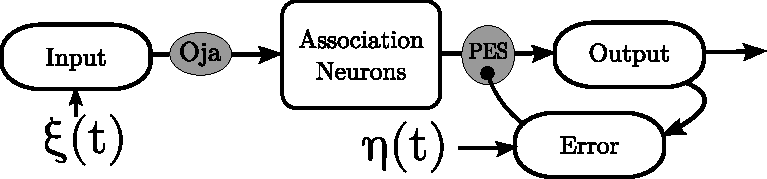
\includegraphics[width=\textwidth]{../diagrams/schematic.pdf}
%\end{center}
\caption{Schematic diagram of association network. White rectangles indicate populations of spiking neurons, arrows indicate all-to-all connections between populations, and grey ellipses indicate learning rules applied to connections.}
\label{fig:schematic}
\end{figure*}

\section{Discussion}
The current study leaves a number of questions unanswered. Future work will investigate whether the learned memory can be mapped to brain structures. Moreover, work will be done to investigate the time course on which presentations to the network should occur, to adhere to data about the manner and rate in which children learn such relations. It would be interesting to see whether different time courses have consequences for what is ultimately learned by the memory. For instance, there is reason to expect such a memory to be able to account for interference effects; if a new item is learned while a similar item is still being recorded, it is a plausible hypothesis that, through Oja's rule, the new item will ``steal'' neurons from the incomplete item, rendering the incomplete item difficult or even impossible to access. This has been observed empirically CITATION. Further simulations will be required to investigate these intriguing questions.

Provides certain self-correcting mechanism.
Moreover.. if you learn one relation at some early point, but then never see that relation again, but do see many other relations, the old one could be cancelled out, which could ultimately be a good thing.. the original one could be cancelled out over time.

One shortcoming of our method is that there is a limit to the number of relations that can be stored in any given vector. This is a consequence of the fact the HRR's compress many vectors of a given dimension into a single vector of the same dimension; obviously if we try to stuff too many vectors into a single HRR, much of the information will be lost. This seems like an important shortcoming, since clearly it is possible to know quite a lot about a given subject; experts abound. Our answer to this challenge is that since our method is so efficient, it is possible to have many of these memories in the brain. Thus as one becomes an expert in a subject, their representations of items will become more fine-grained, all these subtle distinctions being offloaded to another memory in a separate part of the brain. This may explain the commonly observed phenomena that experts have larger brains and more neurons in brain areas that are known to be relevant to their area of expertise CITATION.

See how it applies to learning categories.. like i was working on earlier, clustering and prototypes.

Pattern separation and the identity vectors.
Further explication the form of semantic representations in the brain.. i.e. emprically determing WHAT gets stored. i.e., what exactly are the identity vectors? seems like an important question.

While this has mainly been presented as a theoretical study and a proof of principle, it remains plausible that such a 

Has a lot of flexibility in terms of what can be stored in the HRR's.

Role of neurogenesis, so we don't need a predetermined size of the cleanup pool. 



\section{Conclusion}
Novel combination of synaptic plasticity and distributed vector representations. \textbf{I think this is really the selling point, and what should get the paper noticed}.

\section{Acknowledgments}
Funding for this work was provided by the National Science and Engineering Research Council of Canada, Canada Research Chairs, the Canadian Foundation for Innovation and the Ontario Innovation Trust.		
\bibliographystyle{apacite}

\setlength{\bibleftmargin}{.125in}
\setlength{\bibindent}{-\bibleftmargin}

\bibliography{library}

\end{document}
